%%%%%%%%%%%%%%%%%%%%%%%%%%%%%%%%%%%%%%%%%%%%%%%%%%%%%%%%%%%%%%%%%%%%%%
% LaTeX Template: Beamer arrows
%
% Source: http://www.texample.net/
% Feel free to distribute this template, but please keep the
% referal to TeXample.net.
% Date: Nov 2006
%
%%%%%%%%%%%%%%%%%%%%%%%%%%%%%%%%%%%%%%%%%%%%%%%%%%%%%%%%%%%%%%%%%%%%%%
% How to use writeLaTeX:4
%
% You edit the source code here on the left, and the preview on the
% right shows you the result within a few seconds.
%
% Bookmark this page and share the URL with your co-authors. They can
% edit at the same time!
%
% You can upload figures, bibliographies, custom classes and
% styles using the files menu.
%
% If you're new to LaTeX, the wikibook is a great place to start:
% http://en.wikibooks.org/wiki/LaTeX
%
%%%%%%%%%%%%%%%%%%%%%%%%%%%%%%%%%%%%%%%%%%%%%%%%%%%%%%%%%%%%%%%%%%%%%%

\documentclass{beamer} %
\usetheme{CambridgeUS}
\usepackage[latin1]{inputenc}
\usefonttheme{professionalfonts}
\usepackage{times}
% \usepackage{tikz}
\usepackage{amsmath}
\usepackage{amssymb}
\usepackage{verbatim}
\usepackage{graphicx}
\usepackage{csquotes}
% \usetikzlibrary{arrows,shapes}

\renewcommand{\vec}[1]{\mathbf{#1}}
\DeclareMathOperator{\sign}{sgn}

\DeclareMathOperator{\EX}{\mathbb{E}}

\author{Jo\"el Faubert}
\title{3D Reconstruction with RGB-D Cameras}

\begin{document}

\begin{comment}
:Title: State of the Art on 3D Reconstruction with RGB-D Cameras
:Tags: Project Proposal for COMP5115
:Use page: 3

\end{comment}

\everymath{\displaystyle}

\begin{frame}
%\frametitle{Title}

\begin{center}
{\Large
Pagliari et al.

Kinect Fusion Improvement Using Depth Camera Calibration}

COMP5115 - Fall 2019
\end{center}
\end{frame}

\begin{frame}
\frametitle{Outline}

\begin{itemize}
\item Introduction and Motivation
\item Related Works
\item The KinectFusion Method
\begin{itemize}
  \item Measurement
  \item Surface Reconstruction
  \item Surface Prediction
  \item Sensor Pose Estimation
\end{itemize}
\item Results and Conclusion
\end{itemize}

\end{frame}

\begin{frame}
\frametitle{Introduction and Motivation}

\begin{itemize}
\item Purchased an Intel RealSense D435 Camera.
\item Studied STAR paper by Zollh\"ofer to see how it could be used.
\item Realized that article was too high-level (and advanced).
\item KinectFusion seems to have established current paradigm. Explains math bits nicely,
so a good starting paper.
\end{itemize}
\begin{center}
\includegraphics[scale=0.25]{img/depth_selfie.png}
\end{center}
\end{frame}

\begin{frame}
\frametitle{Problem Statement}

Problem: process a stream of RGB-D frames for Simultaneous Localization and Mapping
(and do it in real time!)

\begin{itemize}
  \item Tracking: estimate the pose (position + orientation) of the camera.
  Camera presumed moving through space -- need to keep track of position and which way it's pointing.
  \item Mapping: (incrementally) build a model of the scene captured by camera.
\end{itemize}
\end{frame}

\begin{frame}
\frametitle{Challenges}
\begin{itemize}
  \item High volume of data (640x480 @ 30fps = 9 million points per sec)
  \item Occlusion (stuff in the way), holes
  \item Measurement errors: incident angles, shiny or transparent materials
  \item Potentially erratic camera movement: blurry measurements
  \item Dynamic scenes, moving objects
  \item Camera drift: accumulation of errors in pose estimation
\end{itemize}
\end{frame}

\begin{frame}[allowframebreaks]
  \frametitle<presentation>{Related Works}
  \begin{thebibliography}{1}
  \beamertemplatearticlebibitems

  \bibitem{beardsley1997sfm}
  \newblock Beardsley, et al. 1997
\newblock Sequential updating of projective and affine structure from motionof projective and affine structure from motion.
  \bibitem{fitzgibbon1998recovery}
  \newblock Fitzgibbon et al. 1998
  \newblock Automatic camera recovery for closed or open image sequences.
  \bibitem{davidson2003slam}
  \newblock A. J. Davison. 2003
  \newblock Real-time simultaneous localisation and mapping with a single camera.
  \bibitem{klein2007ptam}
  \newblock G. Klein and D. W. Murray. 2007
  \newblock Parallel tracking and mapping for small AR workspaces.
  \bibitem{newcombe2010livedense}
  \newblock R. A. Newcombe and A. J. Davison. 2010
  \newblock Live dense reconstruction with a single moving camera.
  \end{thebibliography}
\end{frame}


\begin{frame}
\frametitle{Fusion Methods}
Goal: Reconstruct a global model $\mathbb{M} = (\hat{V}, \hat{N})$ from
a sequence of depth frames $D_i = (V_i, N_i)$. \\

Assuming that the scene is static, depth frames can be fused into a single
point cloud by finding the camera pose which aligns the current depth frame
with the model. \\

Outlier points which do not fit in the model should be presumed errors and discarded.
\end{frame}

\begin{frame}[allowframebreaks]
\frametitle{Challenges}
Measurement
\begin{itemize}
  \item High volume of data (640x480 @ 30fps = 9 million points per sec)
  \item Occlusion (stuff in the way), holes
  \item Measurement errors: incident angles, shiny or transparent materials
  \item Potentially erratic camera movement: blurry measurements
  \item Dynamic scenes, moving objects
  \item Camera drift: accumulation of errors in pose estimation
\end{itemize}
Video: playing with RealSense PointCloud example: \url{https://youtu.be/cQrPQ1dFIYU}
\end{frame}


\begin{frame}[allowframebreaks]
\frametitle{Frameworks}
Fusion and alignment algorithms are bundled in a few frameworks:
\begin{itemize}
  \item Robot Operating System (ROS)
  \item Point Cloud Library
  \item OpenCV (Kinfu)
\end{itemize}

Intel RealSense SDK provides ``wrappers'' for these frameworks.

Idea: encapsulate sensing device so that a stream (or pipe) can be fed into
one of these frameworks' algorithms.

\url{https://github.com/IntelRealSense/librealsense/blob/master/wrappers/opencv/kinfu/rs-kinfu.cpp}
\end{frame}


\section{Results}

An initial goal of this project was to create a model of my head for 3d printing,
but it was difficult to keep a consistent posture for multiple angles.
\begin{figure}[h]
\centering
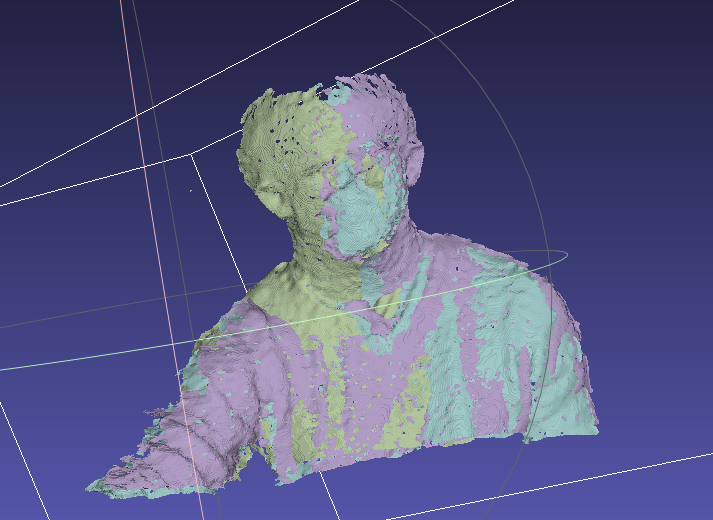
\includegraphics[width=0.6\textwidth]{poor_alignment.png}
\caption{Difficult to take depth selfies from different angles without moving}
\end{figure}
Photography skill (and a longer USB cable!) would be helpful for capturing quality depth images.
When the object is not rigid across different frames the point clouds do not quite fit together.

For the Cube Man project, the final reconstructions are somewhat disappointing.
None of the reconstruction methods tried reconstruct a smooth but detailed model.
Even after carefully aligning multiple clouds the reconstruction obtained
from the merged point clouds is jagged and full of artifacts.

The reality is that these devices do not have very good accuracy at small scales.
The infrared emitter mitigates some of the problems of stereoscopic depth but
also seem to introduce some noise.

However, the D435 and like can produce a stream of decent depth images
at high speed.  Obviously, the Fusion method \cite{newcombe2011kinectfusion}
is superior to this artisanal approach. With a big data streaming approach,
it is possible to identify noise, discard erroneous values and fill in holes and details.


\section{Conclusion}


\begin{frame}[allowframebreaks]
  \frametitle<presentation>{References}
  \begin{thebibliography}{1}
  \beamertemplatearticlebibitems
  \bibitem{zollhofer2018state}
    Zollh{\"o}fer, Michael et al. (2018)
    \newblock State of the Art on 3D Reconstruction with RGB-D Cameras
    \newblock Computer Graphics Forum
  \bibitem{pagliari2014kinect}
    Pagliari, Diana and Menna, Fabio and Roncella, R and Remondino, Fabio and Pinto, Livio (2011)
    \newblock Kinect Fusion improvement using depth camera calibration
    \newblock Photogrammetry, Remote Sensing and Spatial Information Sciences
  \end{thebibliography}
\end{frame}


\end{document}
